%\renewcommand{\theequation}{\theenumi}
%\begin{enumerate}[label=\arabic*.,ref=\thesubsection.\theenumi]
%\numberwithin{equation}{enumi}

\item Solve the following pair of linear equations
%
\begin{enumerate}[itemsep=2pt]
%\begin{enumerate}[itemsep=2pt]
%\begin{multicols}{2}
\item
\begin{align}
\begin{split}
\myvec{p & q }\vec{x}&=p-q
\\
\myvec{q & -p }\vec{x}&=p+q
\end{split}
\end{align}
\item
\begin{align}
\begin{split}
\myvec{a & b }\vec{x}&=c
\\
\myvec{b & a }\vec{x}&=1+c
\end{split}
\end{align}
\item
\begin{align}
\begin{split}
\myvec{\frac{1}{a} & -\frac{1}{b} }\vec{x}&=0
\\
\myvec{a & b }\vec{x}&=a^2+b^2
\end{split}
\end{align}
%
%\end{multicols}
\end{enumerate}
%\solution 
%
General equation of conics is 
\begin{align}
    \vec{x}^T\vec{V}\vec{x}+ 2\vec{u}^T\vec{x}+f = 0
    \label{eq:solutions/1/16/eq:1}
\end{align}
Comparing with the equation given,
\begin{align}
\vec{V}=\myvec{\frac{1}{9} & 0 \\ 0 & \frac{1}{16}}\\
\vec{u}=\vec{0}\\
f=-1\\
\mydet{\vec{v}}=\mydet{\myvec{\frac{1}{9} & 0 \\ 0 & \frac{1}{16}}}>0
\end{align}
$\because \abs{\vec{V}}>0$, the given equation is of ellipse.\\
a)The tangents are parallel to the x-axis, hence, their direction and normal vectors, $\vec{m_1}$ and $\vec{n_1}$ are respectively,
\begin{align}
\vec{m_1}=\myvec{1\\0}\\
\vec{n_1}=\myvec{0\\1}
\end{align}
For an ellipse, given the normal vector $\vec{n}$, the tangent points of contact to the ellipse are given by
\begin{align}
    \vec{q}=\vec{V}^{-1}(\kappa \vec{n}-\vec{u})
    \label{eq:solutions/1/16/eq:2}
    =\vec{V}^{-1}\kappa \vec{n}
\end{align}
where
\begin{align}
    \kappa=\pm \sqrt{\frac{\vec{u^T}\vec{V}^{-1}\vec{u}-f}{\vec{n^T}\vec{V}^{-1}\vec{n}}}
    \label{eq:solutions/1/16/eq:2.0.9}\\
   =\pm \sqrt{\frac{-f}{\vec{n^T}\vec{V}^{-1}\vec{n}}}\\
    \vec{V}^{-1}=\myvec{9 & 0 \\ 0 & 16}\\
    \kappa_1=\pm \sqrt{\frac{-(-1)}{\myvec{0 & 1}\myvec{9 & 0 \\ 0 & 16} \myvec{0\\1}}}\\
 \implies \kappa_1=\pm \sqrt{\frac{1}{16}}\\
    \implies \kappa_1=\pm \frac{1}{4}      
\end{align}
From \eqref{eq:solutions/1/16/eq:2} , the point of contact $\vec{q_i}$ are,
\begin{align}
    \vec{q_1}=\myvec{9 & 0 \\ 0 & 16}\frac{1}{4}\myvec{0\\1}\\
    =\myvec{9 & 0 \\ 0 & 16}\myvec{0\\\frac{1}{4}}\\
    =\myvec{0\\4}\\
    \vec{q_2}=\myvec{9 & 0 \\ 0 & 16}\left(-\frac{1}{4}\right)\ \myvec{0\\1}\\
    =\myvec{9 & 0 \\ 0 & 16}\myvec{0\\-\frac{1}{4}}\\
    =\myvec{0\\-4}
\end{align}
b) The tangents are parallel to the y-axis, hence, their direction and normal vectors, $\vec{m_2}$ and $\vec{n_2}$ are respectively,
\begin{align}
\vec{m_2}=\myvec{0\\1}\\
\vec{n_2}=\myvec{1\\0}
\end{align}
Using equation \eqref{eq:solutions/1/16/eq:2.0.9}, the values of $\kappa$ for this case are
\begin{align}
     \kappa_2=\pm \sqrt{\frac{-(-1)}{\myvec{1 & 0}\myvec{9 & 0 \\ 0 & 16} \myvec{1\\0}}}\\
 \implies \kappa_2=\pm \sqrt{\frac{1}{9}}\\
    \implies \kappa_2=\pm \frac{1}{3} 
\end{align}
and from \eqref{eq:solutions/1/16/eq:2} , the point of contact $\vec{q_i}$ are,
\begin{align}
\vec{q_3}=\myvec{9 & 0 \\ 0 & 16}\frac{1}{3}\myvec{1\\0}\\
    =\myvec{9 & 0 \\ 0 & 16}\myvec{\frac{1}{3}\\0}\\
    =\myvec{3\\0}\\
\vec{q_4}=\myvec{9 & 0 \\ 0 & 16}\left(-\frac{1}{3}\right)\ \myvec{1\\0}\\
    =\myvec{9 & 0 \\ 0 & 16}\myvec{-\frac{1}{3}\\0}\\
    =\myvec{-3\\0}
\end{align}
 \begin{figure}[h!]
	\centering
	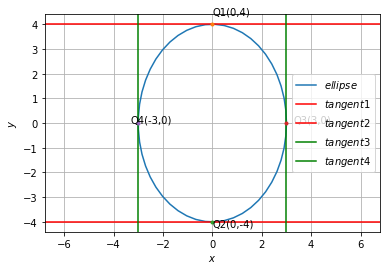
\includegraphics[width=\columnwidth]{./solutions/conics/1/16/ellipse.png}
	\caption{Figure depicting point of contact of tangents of ellipse parallel to x-axis and y-axis}
	\label{eq:solutions/1/16/fig1}
\end{figure}

%
\item Solve the following pair of equations
\begin{align}
\begin{split}
\myvec{a-b & a+b }\vec{x}&=a^2-2ab-b^2
\\
\myvec{a+b & a+b }\vec{x}&=a^2+b^2
\end{split}
\end{align}
%\solution 
%
General equation of conics is 
\begin{align}
    \vec{x}^T\vec{V}\vec{x}+ 2\vec{u}^T\vec{x}+f = 0
    \label{eq:solutions/1/16/eq:1}
\end{align}
Comparing with the equation given,
\begin{align}
\vec{V}=\myvec{\frac{1}{9} & 0 \\ 0 & \frac{1}{16}}\\
\vec{u}=\vec{0}\\
f=-1\\
\mydet{\vec{v}}=\mydet{\myvec{\frac{1}{9} & 0 \\ 0 & \frac{1}{16}}}>0
\end{align}
$\because \abs{\vec{V}}>0$, the given equation is of ellipse.\\
a)The tangents are parallel to the x-axis, hence, their direction and normal vectors, $\vec{m_1}$ and $\vec{n_1}$ are respectively,
\begin{align}
\vec{m_1}=\myvec{1\\0}\\
\vec{n_1}=\myvec{0\\1}
\end{align}
For an ellipse, given the normal vector $\vec{n}$, the tangent points of contact to the ellipse are given by
\begin{align}
    \vec{q}=\vec{V}^{-1}(\kappa \vec{n}-\vec{u})
    \label{eq:solutions/1/16/eq:2}
    =\vec{V}^{-1}\kappa \vec{n}
\end{align}
where
\begin{align}
    \kappa=\pm \sqrt{\frac{\vec{u^T}\vec{V}^{-1}\vec{u}-f}{\vec{n^T}\vec{V}^{-1}\vec{n}}}
    \label{eq:solutions/1/16/eq:2.0.9}\\
   =\pm \sqrt{\frac{-f}{\vec{n^T}\vec{V}^{-1}\vec{n}}}\\
    \vec{V}^{-1}=\myvec{9 & 0 \\ 0 & 16}\\
    \kappa_1=\pm \sqrt{\frac{-(-1)}{\myvec{0 & 1}\myvec{9 & 0 \\ 0 & 16} \myvec{0\\1}}}\\
 \implies \kappa_1=\pm \sqrt{\frac{1}{16}}\\
    \implies \kappa_1=\pm \frac{1}{4}      
\end{align}
From \eqref{eq:solutions/1/16/eq:2} , the point of contact $\vec{q_i}$ are,
\begin{align}
    \vec{q_1}=\myvec{9 & 0 \\ 0 & 16}\frac{1}{4}\myvec{0\\1}\\
    =\myvec{9 & 0 \\ 0 & 16}\myvec{0\\\frac{1}{4}}\\
    =\myvec{0\\4}\\
    \vec{q_2}=\myvec{9 & 0 \\ 0 & 16}\left(-\frac{1}{4}\right)\ \myvec{0\\1}\\
    =\myvec{9 & 0 \\ 0 & 16}\myvec{0\\-\frac{1}{4}}\\
    =\myvec{0\\-4}
\end{align}
b) The tangents are parallel to the y-axis, hence, their direction and normal vectors, $\vec{m_2}$ and $\vec{n_2}$ are respectively,
\begin{align}
\vec{m_2}=\myvec{0\\1}\\
\vec{n_2}=\myvec{1\\0}
\end{align}
Using equation \eqref{eq:solutions/1/16/eq:2.0.9}, the values of $\kappa$ for this case are
\begin{align}
     \kappa_2=\pm \sqrt{\frac{-(-1)}{\myvec{1 & 0}\myvec{9 & 0 \\ 0 & 16} \myvec{1\\0}}}\\
 \implies \kappa_2=\pm \sqrt{\frac{1}{9}}\\
    \implies \kappa_2=\pm \frac{1}{3} 
\end{align}
and from \eqref{eq:solutions/1/16/eq:2} , the point of contact $\vec{q_i}$ are,
\begin{align}
\vec{q_3}=\myvec{9 & 0 \\ 0 & 16}\frac{1}{3}\myvec{1\\0}\\
    =\myvec{9 & 0 \\ 0 & 16}\myvec{\frac{1}{3}\\0}\\
    =\myvec{3\\0}\\
\vec{q_4}=\myvec{9 & 0 \\ 0 & 16}\left(-\frac{1}{3}\right)\ \myvec{1\\0}\\
    =\myvec{9 & 0 \\ 0 & 16}\myvec{-\frac{1}{3}\\0}\\
    =\myvec{-3\\0}
\end{align}
 \begin{figure}[h!]
	\centering
	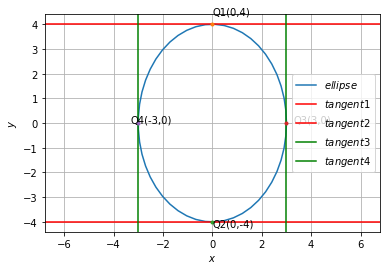
\includegraphics[width=\columnwidth]{./solutions/conics/1/16/ellipse.png}
	\caption{Figure depicting point of contact of tangents of ellipse parallel to x-axis and y-axis}
	\label{eq:solutions/1/16/fig1}
\end{figure}


\item In $\triangle ABC$, Show that the centroid 
\begin{align}
\vec{O} = \frac{\vec{A}+\vec{B}+\vec{C}}{3}
\end{align}
%
%\\
%\solution 
%\renewcommand{\theequation}{\theenumi}
\begin{enumerate}[label=\thesection.\arabic*.,ref=\thesection.\theenumi]
\numberwithin{equation}{enumi}
\item Let the medians $BE$ and $CF$ in Fig. \ref{fig:3.12.3_ch1_two_median} intersect at $O$, such that
\begin{equation}
\begin{split}
\frac{OB}{OE} &= k_1
\\
\frac{OC}{OF} &= k_2
\end{split}
\end{equation}
%Then  $k_1 = k_2 = 2$.
%
\begin{figure}[!h]
\centering
\resizebox {\columnwidth} {!} {
\begin{tikzpicture}
  [
    scale=2,
    >=stealth,
    point/.style = {draw, circle,  fill = black, inner sep = 0.5pt},
    dot/.style   = {draw, circle,  fill = black, inner sep = .2pt},
  ]
  \coordinate [point, label={below left:$B$ $(0, 0)$}] (B) at (0, 0);
    \node (A) at +(60:{2*sqrt(3)}) [point, label = above:$A$ ${(a,b)}$  ] {};
  \coordinate [point, label={below left:$(c,0)$ $C$ }] (C) at ($ (3,0) + sqrt(3)*(1,0) $);

  \draw  (A) -- (C) -- (B) -- (A);
  \node (E) at ($(A)!0.5!(C)$) [point, label = {right:$E$}]{};
  \node (F) at ($(A)!0.5!(B)$) [point, label = {left:$F$}]{};
  \path
     (B)    edge  node[sloped, anchor=center, below, text width=2.0cm] { $k_1:1$}     (E)  
	 (C)    edge  node[sloped, anchor=east, below, text width=2.0cm] { $1:k_2$}     (F);
  \node (O) at ($(B)!0.67!(E)$) [point, label = {below:$O$}]{};  
\end{tikzpicture}


}
\caption{Medians $BE$ and $CF$}
\label{fig:3.12.3_ch1_two_median}
\end{figure}
%Let the coordinates of $A$, $B$ and $C$ be $\brak{a,b}$, $\brak{0,0}$ and $\brak{c,0}$ respectively. 
Using \eqref{eq:line_section_form},
%
\begin{align}
E &= \frac{\vec{A}+\vec{C}}{2} 
\\
F &= \frac{\vec{A}+\vec{B}}{2} 
\label{eq:3.12.3_ch1_ratio_ef}
\end{align}
%
Similarly, since $O$ divides $BE$ in the ratio $k_1:1$ and $CF$ in the ratio $k_2:1$.
 %
\begin{align}
O = \frac{k_1\vec{E}+\vec{B}}{k_1+1} &=  \frac{k_2\vec{F}+\vec{C}}{k_2+1} 
\\
\implies \frac{k_1\brak{\frac{\vec{A}+\vec{C}}{2}} +B}{k_1+1} &=  \frac{k_2\brak{\frac{\vec{A}+\vec{B}}{2} }+C}{k_2+1} 
\label{eq:3.12.3_ch1_ratio_2}
\end{align}
upon substituting from \eqref{eq:3.12.3_ch1_ratio_ef}.
Simplifying \eqref{eq:3.12.3_ch1_ratio_2},
\begin{align}
\frac{k_1\brak{\vec{A}+\vec{C}} +2\vec{B}}{k_1+1} =  \frac{k_2\brak{\vec{A}+\vec{B}}+2\vec{C}}{k_2+1} 
\end{align}
which can be expressed as
\begin{multline}
\implies \sbrak{k_1\brak{k_2+1}-k_2\brak{k_1+1}}\vec{A}
\\
 +\sbrak{2\brak{k_2+1}-k_2\brak{k_1+1}}\vec{B}
\\ +  \sbrak{k_1\brak{k_2+1} -2\brak{k_1+1}}\vec{C} = 0
\end{multline}
resulting in 
\begin{align}
\vec{B} = \frac{\brak{k_1-k_2}\vec{A}+\brak{k_1k_2 -k_1 -2}}{k_1k_2 -k_2 -2}
\end{align}
%
If the above equation has a solution, then $\vec{A}, \vec{B}$ and $\vec{C}$ lie on a straight line.  Since that is not the case, the only possibility is 
\begin{align}
k_1-k_2 &= 0
\\
k_1k_2 -k_1 -2 &= 0
\\
k_1k_2 -k_2 -2 &= 0
\\
\implies k_1=k_2&=2
\end{align}
{\em If $\vec{A}, \vec{B}, \vec{C}$ lie on a triangle, they are linearly independent.}    In which case, 
\begin{align}
x_1\vec{A}+ x_2\vec{B}+x_3\vec{C} &= 0
\\
\implies x_1 = x_2=x_3 = 0,
\end{align}
Else, they are linearly dependent and lie on a straight line.
\item In Fig. \ref{fig:3.12.3_ch1_two_median},
\begin{align}
\vec{E} &=  \frac{\vec{A}+\vec{C}}{2} \quad \text{and}
\\
\vec{O}&= \frac{\vec{B}+2\vec{E}}{3}
\\
&= \frac{\vec{A}+\vec{B}+\vec{C}}{3}
\end{align}
\end{enumerate}
	


%\item (Cauchy-Schwarz Inequality:) Show that 
%%
%\begin{align}
%\abs{\vec{a}^T\vec{b}} \le \norm{\vec{a}}\norm{\vec{b}}
%\end{align}
%%
%\solution 
%
General equation of conics is 
\begin{align}
    \vec{x}^T\vec{V}\vec{x}+ 2\vec{u}^T\vec{x}+f = 0
    \label{eq:solutions/1/16/eq:1}
\end{align}
Comparing with the equation given,
\begin{align}
\vec{V}=\myvec{\frac{1}{9} & 0 \\ 0 & \frac{1}{16}}\\
\vec{u}=\vec{0}\\
f=-1\\
\mydet{\vec{v}}=\mydet{\myvec{\frac{1}{9} & 0 \\ 0 & \frac{1}{16}}}>0
\end{align}
$\because \abs{\vec{V}}>0$, the given equation is of ellipse.\\
a)The tangents are parallel to the x-axis, hence, their direction and normal vectors, $\vec{m_1}$ and $\vec{n_1}$ are respectively,
\begin{align}
\vec{m_1}=\myvec{1\\0}\\
\vec{n_1}=\myvec{0\\1}
\end{align}
For an ellipse, given the normal vector $\vec{n}$, the tangent points of contact to the ellipse are given by
\begin{align}
    \vec{q}=\vec{V}^{-1}(\kappa \vec{n}-\vec{u})
    \label{eq:solutions/1/16/eq:2}
    =\vec{V}^{-1}\kappa \vec{n}
\end{align}
where
\begin{align}
    \kappa=\pm \sqrt{\frac{\vec{u^T}\vec{V}^{-1}\vec{u}-f}{\vec{n^T}\vec{V}^{-1}\vec{n}}}
    \label{eq:solutions/1/16/eq:2.0.9}\\
   =\pm \sqrt{\frac{-f}{\vec{n^T}\vec{V}^{-1}\vec{n}}}\\
    \vec{V}^{-1}=\myvec{9 & 0 \\ 0 & 16}\\
    \kappa_1=\pm \sqrt{\frac{-(-1)}{\myvec{0 & 1}\myvec{9 & 0 \\ 0 & 16} \myvec{0\\1}}}\\
 \implies \kappa_1=\pm \sqrt{\frac{1}{16}}\\
    \implies \kappa_1=\pm \frac{1}{4}      
\end{align}
From \eqref{eq:solutions/1/16/eq:2} , the point of contact $\vec{q_i}$ are,
\begin{align}
    \vec{q_1}=\myvec{9 & 0 \\ 0 & 16}\frac{1}{4}\myvec{0\\1}\\
    =\myvec{9 & 0 \\ 0 & 16}\myvec{0\\\frac{1}{4}}\\
    =\myvec{0\\4}\\
    \vec{q_2}=\myvec{9 & 0 \\ 0 & 16}\left(-\frac{1}{4}\right)\ \myvec{0\\1}\\
    =\myvec{9 & 0 \\ 0 & 16}\myvec{0\\-\frac{1}{4}}\\
    =\myvec{0\\-4}
\end{align}
b) The tangents are parallel to the y-axis, hence, their direction and normal vectors, $\vec{m_2}$ and $\vec{n_2}$ are respectively,
\begin{align}
\vec{m_2}=\myvec{0\\1}\\
\vec{n_2}=\myvec{1\\0}
\end{align}
Using equation \eqref{eq:solutions/1/16/eq:2.0.9}, the values of $\kappa$ for this case are
\begin{align}
     \kappa_2=\pm \sqrt{\frac{-(-1)}{\myvec{1 & 0}\myvec{9 & 0 \\ 0 & 16} \myvec{1\\0}}}\\
 \implies \kappa_2=\pm \sqrt{\frac{1}{9}}\\
    \implies \kappa_2=\pm \frac{1}{3} 
\end{align}
and from \eqref{eq:solutions/1/16/eq:2} , the point of contact $\vec{q_i}$ are,
\begin{align}
\vec{q_3}=\myvec{9 & 0 \\ 0 & 16}\frac{1}{3}\myvec{1\\0}\\
    =\myvec{9 & 0 \\ 0 & 16}\myvec{\frac{1}{3}\\0}\\
    =\myvec{3\\0}\\
\vec{q_4}=\myvec{9 & 0 \\ 0 & 16}\left(-\frac{1}{3}\right)\ \myvec{1\\0}\\
    =\myvec{9 & 0 \\ 0 & 16}\myvec{-\frac{1}{3}\\0}\\
    =\myvec{-3\\0}
\end{align}
 \begin{figure}[h!]
	\centering
	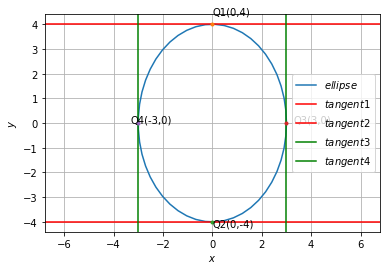
\includegraphics[width=\columnwidth]{./solutions/conics/1/16/ellipse.png}
	\caption{Figure depicting point of contact of tangents of ellipse parallel to x-axis and y-axis}
	\label{eq:solutions/1/16/fig1}
\end{figure}

%%
%\item (Triangle Inequality:) Show that 
%%
%\begin{align}
%\norm{\vec{a}+\vec{b}} \le \norm{\vec{a}}+\norm{\vec{b}}
%\end{align}
%%
%\solution 
%	\begin{align}
		\norm{\vec{a}+\vec{b}}^2 &= \norm{\vec{a}}^2+2\vec{a}^T\vec{b}+\norm{\vec{b}}^2\\
&\le \norm{\vec{a}}^2+2\norm{\vec{a}}\norm{\vec{b}}+\norm{\vec{b}}^2\\
\implies 	\norm{\vec{a}+\vec{b}}^2 &\leq \brak{\norm{\vec{a}} + \norm{\vec{b}}}^2\\
\text{or, }		\norm{\vec{a}+\vec{b}} &\le  \norm{\vec{a}} + \norm{\vec{b}}
	\end{align}
using Cauchy-Schwarz inequality.

%
\item The base of an equilateral triangle with side $2a$ lies along the y-axis such that the mid-point of the base is at the origin. Find vertices of the triangle.
%\solution 
%
General equation of conics is 
\begin{align}
    \vec{x}^T\vec{V}\vec{x}+ 2\vec{u}^T\vec{x}+f = 0
    \label{eq:solutions/1/16/eq:1}
\end{align}
Comparing with the equation given,
\begin{align}
\vec{V}=\myvec{\frac{1}{9} & 0 \\ 0 & \frac{1}{16}}\\
\vec{u}=\vec{0}\\
f=-1\\
\mydet{\vec{v}}=\mydet{\myvec{\frac{1}{9} & 0 \\ 0 & \frac{1}{16}}}>0
\end{align}
$\because \abs{\vec{V}}>0$, the given equation is of ellipse.\\
a)The tangents are parallel to the x-axis, hence, their direction and normal vectors, $\vec{m_1}$ and $\vec{n_1}$ are respectively,
\begin{align}
\vec{m_1}=\myvec{1\\0}\\
\vec{n_1}=\myvec{0\\1}
\end{align}
For an ellipse, given the normal vector $\vec{n}$, the tangent points of contact to the ellipse are given by
\begin{align}
    \vec{q}=\vec{V}^{-1}(\kappa \vec{n}-\vec{u})
    \label{eq:solutions/1/16/eq:2}
    =\vec{V}^{-1}\kappa \vec{n}
\end{align}
where
\begin{align}
    \kappa=\pm \sqrt{\frac{\vec{u^T}\vec{V}^{-1}\vec{u}-f}{\vec{n^T}\vec{V}^{-1}\vec{n}}}
    \label{eq:solutions/1/16/eq:2.0.9}\\
   =\pm \sqrt{\frac{-f}{\vec{n^T}\vec{V}^{-1}\vec{n}}}\\
    \vec{V}^{-1}=\myvec{9 & 0 \\ 0 & 16}\\
    \kappa_1=\pm \sqrt{\frac{-(-1)}{\myvec{0 & 1}\myvec{9 & 0 \\ 0 & 16} \myvec{0\\1}}}\\
 \implies \kappa_1=\pm \sqrt{\frac{1}{16}}\\
    \implies \kappa_1=\pm \frac{1}{4}      
\end{align}
From \eqref{eq:solutions/1/16/eq:2} , the point of contact $\vec{q_i}$ are,
\begin{align}
    \vec{q_1}=\myvec{9 & 0 \\ 0 & 16}\frac{1}{4}\myvec{0\\1}\\
    =\myvec{9 & 0 \\ 0 & 16}\myvec{0\\\frac{1}{4}}\\
    =\myvec{0\\4}\\
    \vec{q_2}=\myvec{9 & 0 \\ 0 & 16}\left(-\frac{1}{4}\right)\ \myvec{0\\1}\\
    =\myvec{9 & 0 \\ 0 & 16}\myvec{0\\-\frac{1}{4}}\\
    =\myvec{0\\-4}
\end{align}
b) The tangents are parallel to the y-axis, hence, their direction and normal vectors, $\vec{m_2}$ and $\vec{n_2}$ are respectively,
\begin{align}
\vec{m_2}=\myvec{0\\1}\\
\vec{n_2}=\myvec{1\\0}
\end{align}
Using equation \eqref{eq:solutions/1/16/eq:2.0.9}, the values of $\kappa$ for this case are
\begin{align}
     \kappa_2=\pm \sqrt{\frac{-(-1)}{\myvec{1 & 0}\myvec{9 & 0 \\ 0 & 16} \myvec{1\\0}}}\\
 \implies \kappa_2=\pm \sqrt{\frac{1}{9}}\\
    \implies \kappa_2=\pm \frac{1}{3} 
\end{align}
and from \eqref{eq:solutions/1/16/eq:2} , the point of contact $\vec{q_i}$ are,
\begin{align}
\vec{q_3}=\myvec{9 & 0 \\ 0 & 16}\frac{1}{3}\myvec{1\\0}\\
    =\myvec{9 & 0 \\ 0 & 16}\myvec{\frac{1}{3}\\0}\\
    =\myvec{3\\0}\\
\vec{q_4}=\myvec{9 & 0 \\ 0 & 16}\left(-\frac{1}{3}\right)\ \myvec{1\\0}\\
    =\myvec{9 & 0 \\ 0 & 16}\myvec{-\frac{1}{3}\\0}\\
    =\myvec{-3\\0}
\end{align}
 \begin{figure}[h!]
	\centering
	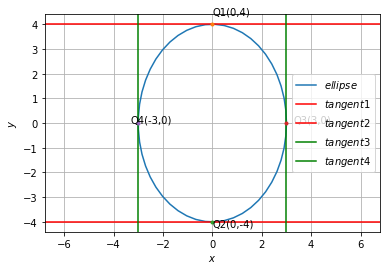
\includegraphics[width=\columnwidth]{./solutions/conics/1/16/ellipse.png}
	\caption{Figure depicting point of contact of tangents of ellipse parallel to x-axis and y-axis}
	\label{eq:solutions/1/16/fig1}
\end{figure}

\item Find the distance between $\vec{P}= \myvec{x_1 y_1}$ and $\vec{Q} =\myvec{x_2 y_2}$ when
\begin{enumerate}
\item PQ is parallel to the y-axis.
\item PQ is parallel to the x-axis.
\end{enumerate}
\item If three points \myvec{h 0}, \myvec{a b} and \myvec{0 k} lie on a line, show that
$\frac{a}{h}+\frac{b}{k}= 1$.
\item $\vec{P}=\myvec{a b}$ is the mid-point of a line segment between axes. Show that equation of the line is
\begin{align}
\myvec{\frac{1}{a} & \frac{1}{b}}\vec{x} = 2
\end{align}
\item  Point $\vec{R}= \myvec{h k}$ divides a line segment between the axes in the ratio 1: 2. Find equation of the line.
\item Show that two lines 
\begin{align}
\myvec{a_1 & b_1}\vec{x} +c_1&= 0
\\
\myvec{a_2 & b_2}\vec{x} +c_2&= 0
\end{align}
are 
\begin{enumerate}
\item parallel if $\frac{a_1}{b_1}=\frac{a_2}{b_2}$ and
\item perpendicular if $a_1a_2-b_1b_2 = 0$.
\end{enumerate}
%
\item Find the distance between the parallel lines
%
\begin{align}
l\myvec{1 & 1}\vec{x} = -p
\\
l\myvec{1 & 1}\vec{x} = r
\end{align}
%
\item Find th equation of the line through the point $\vec{x}_1$ and parallel to the line
%
\begin{align}
\myvec{A & B}\vec{x} = -C
\end{align}
%
\item If $p$ and $q$ are the lengths of perpendiculars from the origin to the lines 
%
\begin{align}
\myvec{\cos\theta & \sin\theta}\vec{x} &= k\cos2\theta
\\
\myvec{\sec\theta & \cosec\theta}\vec{x} &= k
\end{align}
%
respectively, prove that $p^2+4q^2=k^2$.
\item If $p$ is the length of the perpendicular from the origin to the line whose intercepts on the axes are $a$ and $b$, then show that 
%
\begin{align}
\frac{1}{p^2} = \frac{1}{a^2}+\frac{1}{b^2}.
\end{align}
%
\item Show that the area of the triangle formed by the lines
%
\begin{align}
\myvec{-m_1 & 1}\vec{x} = c_1
\\
\myvec{-m_2 & 1}\vec{x} = c_2
\\
\myvec{1 & 0}\vec{x} = 0
\end{align}
%
is $\frac{\brak{c_1-c_2}^2}{2\abs{m_1-m_2}}$.
\item Find the values of $k$ for which the line 
%
\begin{align}
\myvec{k-3 & -\brak{4-k^2}}\vec{x} +k^2-7k+6= 0
\end{align}
%
is
\begin{enumerate}
\item parallel to the x-axis
\item parallel to the y-axis
\item passing through the origin.
\end{enumerate}
%
\item Find the perpendicular distance from the origin to the line joining the points \myvec{\cos\theta\sin\theta} and \myvec{\cos\phi \sin \phi}.
\item Find the area of the triangle formed by the lines
%
\begin{align}
\myvec{1 & -1}\vec{x} &= 0
\\
\myvec{1 & 1}\vec{x} &= 0
\\
\myvec{1 & 0}\vec{x} &= k
\end{align}
%
\item If three lines whose equations are 
%
\begin{align}
\myvec{-m_1 & 1}\vec{x} &= c_1
\\
\myvec{-m_2 & 1}\vec{x} &= c_2
\\
\myvec{-m_3 & 1}\vec{x} &= c_3
\end{align}
%
are concurrent, show that
%
\begin{align}
m_1\brak{c_2-c_3}+
m_2\brak{c_3-c_1}+
m_3\brak{c_1-c_2} = 0
\end{align}
%
\item Find the equation of the line passing through the origin and making an angle $\theta$ with the line %
\begin{align}
\myvec{-m & 1}\vec{x} &= c
\end{align}
%
\item Prove that the product of the lengths of the perpendiculars drawn from the points $\myvec{\sqrt{a^2-b^2}0}$ and $\myvec{\sqrt{a^2-b^2}0}$ to the line 
%
\begin{align}
\myvec{\frac{\cos\theta}{a} & \frac{\sin\theta}{b}}\vec{x} &= 1
\end{align}
%
is $b^2$.

\item If 
$
\myvec{l_1m_1n_1}
$
and
$
\myvec{l_2m_2n_2}
$
are the unit direction vectors of two mutually perpendicular lines, the shown that the unit direction vector of the line perpendicular to both of these is
$
\myvec{m_1n_2-m_2n_1n_1l_2-n_2l_1l_1m_2-l_2m_1}.
$
\item A line makes angles $\alpha, \beta, \gamma, \delta$ with the diagonals of a cube, prove that \begin{align}
\cos^2\alpha + \cos^2\beta + \cos^2\gamma +\cos^2\delta = \frac{4}{3}.
\end{align}
\item Show that the lines 
\begin{align}
\frac{x-a+d}{\alpha-\delta} = \frac{y-a}{\alpha} &= \frac{z-a-d}{\alpha+\delta}, 
\\
\frac{x-b+c}{\beta-\gamma} = \frac{y-b}{\beta} &= \frac{z-b-c}{\beta+\gamma} 
\end{align}
%
are coplanar.
\item Find $\vec{R}$ which divides the line joining the points 
\begin{align}
\vec{P} = 2\vec{a}+\vec{b}
\\
\vec{Q} = \vec{a}-\vec{b}
\end{align}
externally in the ratio $1:2$.
\item Find $\norm{\vec{a}}$ and $\norm{\vec{b}}$ if 
\begin{align}
\brak{\vec{a}+\vec{b}}^T\brak{\vec{a}-\vec{b}} &= 8
\\
\norm{\vec{a}}&=8\norm{\vec{b}}
\end{align}
\item Evaluate the product 
\begin{align}
\brak{3\vec{a}-5\vec{b}}^T\brak{2\vec{a}+7\vec{b}} 
\end{align}
\item Find $\norm{\vec{a}}$ and $\norm{\vec{b}}$, if
\begin{align}
\norm{\vec{a}} &= \norm{\vec{b}},
\\
\vec{a}^T\vec{b} = \frac{1}{2} 
\end{align}
and the angle between $\vec{a}$ and $\vec{b}$ is $60\degree$.
\item Show that 
\begin{align}
\brak{\norm{\vec{a}}\vec{b}+\norm{\vec{b}}\vec{a}}\perp \brak{\norm{\vec{a}}\vec{b}-\norm{\vec{b}}\vec{a}}\\
\end{align}
\item If $\vec{a}^T\vec{a}=0$ and  $\vec{a}\vec{b}=0$, what can be concluded about the vector $\vec{b}$?
\item If $\vec{a},\vec{b},\vec{c}$ are unit vectors such that 
\begin{align}
\vec{a}+\vec{b}+\vec{c} = 0,
\end{align}
find the value of 
\begin{align}
\vec{a}^T\vec{b}+\vec{b}^T\vec{c}+\vec{c}^T\vec{a}.
\end{align}
\item If $\vec{a} \ne \vec{0}, \lambda \ne 0$, then $\norm{\lambda \vec{a}} = 1$ if
\begin{enumerate}
\item $\lambda =1$
\item $\lambda = -1$
\item $\norm{\vec{a}}=\abs{\lambda}$
\item $\norm{\vec{a}}=\frac{1}{\abs{\lambda}}$
\end{enumerate}
\item If a unit vector $\vec{a}$ makes angles $\frac{\pi}{3}$ with the x-axis and $\frac{\pi}{4}$ with the y-axis and an acute angle $\theta$ with the z-axis, find $\theta$ and $\vec{a}$.
\item Show that 
\begin{align}
\brak{\vec{a}-\vec{b}}\times \brak{\vec{a}+\vec{b}} = 2\brak{\vec{a}\times\vec{b}}
\end{align}
\item If $\vec{a}^T\vec{b} = 0$ and $\vec{a}\times \vec{b}$ = 0, what can you conclude about $\vec{a}$ and $\vec{b}$?
\item Find $\vec{x}$ if  $\vec{a}$ is a unit vector such that
\begin{align}
\brak{\vec{x}-\vec{a}}^T\brak{\vec{x}+\vec{a}} = 12.
\end{align}
\item If $\norm{\vec{a}} = 3, \norm{\vec{b}} =\frac{\sqrt{2}}{3}$, then $\vec{a}\times \vec{b}$ is a unit vector if the angle between $\vec{a}$ and $\vec{b}$ is 
\begin{enumerate}[itemsep = 2pt]
\begin{multicols}{2}
\item $\frac{\pi}{6}$
\item $\frac{\pi}{4}$
\item $\frac{\pi}{3}$
\item $\frac{\pi}{2}$
\end{multicols}
\end{enumerate}
\item Prove that 
\begin{align}
\brak{\vec{a}+\vec{b}}^T\brak{\vec{a}+\vec{b}} &= \norm{\vec{a}}^2+\norm{\vec{b}}^2
\\
\iff \vec{a}&\perp\vec{b}.
\end{align}
\item If $\theta$ is the angle between two vectors $\vec{a}$ and $\vec{b}$, then $\vec{a}^T\vec{b} \ge $ only when 
\begin{enumerate}[itemsep = 2pt]
\begin{multicols}{2}
\item $0 < \theta < \frac{\pi}{2}$
\item $0 \le \theta \le \frac{\pi}{2}$
\item $0 < \theta < {\pi}$
\item $0 \le \theta \le {\pi}$
\end{multicols}
\end{enumerate}
\item Let $\vec{a}$ and $\vec{b}$ be two unit vectors and $\theta$ be the angle between them.  Then $\vec{a}+\vec{b}$ is a unit vector if 
\begin{enumerate}[itemsep = 2pt]
\begin{multicols}{2}
\item $\theta = \frac{\pi}{4}$
\item $\theta = \frac{\pi}{3}$
\item $\theta = \frac{\pi}{2}$
\item $\theta = \frac{2\pi}{3}$
\end{multicols}
\end{enumerate}
\item If $\theta$ is the angle between any two vectors $\vec{a}$ and $\vec{b}$, then 
$\norm{\vec{a}^T\vec{b}} = \norm{\vec{a} \times \vec{b}}$ when $\theta$ is equal to 
\begin{enumerate}[itemsep = 2pt]
\begin{multicols}{2}
\item 0
\item $\frac{\pi}{4}$
\item $\frac{\pi}{2}$
\item $\pi$.
\end{multicols}
\end{enumerate}
\item Find the angle between the lines whose direction vectors are $\myvec{abc}$ and $\myvec{b-cc-aa-b}$.
\item Find the equation of a line parallel to the x-axis and passing through the origin.
\item Find the equation of a plane passing through \myvec{abc} and parallel to the plane 
%
\begin{align}
\myvec{1 & 1 & 1}\vec{x}{x}&=2
\end{align}
%
\item Prove that if a plane has the intercepts $a, b, c$ and is at a distance of $p$ units from the origin, then, 
\begin{align}
\frac{1}{a^2}+\frac{1}{b^2}+\frac{1}{c^2}=\frac{1}{p^2} 
\end{align}
     \item In an experiment, a solution of hydrochloric acid is to be kept between 30$\degree$ and 35$\degree$ Celsius. What is the range of temperature in degree Fahrenheit if conversion formula is given by 
     C = $\frac{5}{9}(F-32)$, where C and F represent temperature in degree Celsius and degree Fahrenheit, respectively.
     \item A manufacturer has 600 litres of a 12$\%$ solution of acid. How many litres of a 30$\%$ acid solution must be added to it so that acid content in the resulting mixture will be more than 15$\%$ but less than 18$\%$?
    \item Ravi obtained 70 and 75 marks in first two unit test. Find the minimum marks he should get in the third test to have an average of at least 60 marks.
    \item To receive Grade A in a course, one must obtain an average of 90 marks or more in five examinations (each of 100 marks). If Sunita’s marks in first four examinations are 87, 92, 94 and 95, find minimum marks that Sunita must obtain in fifth examination to get grade ‘A’ in the course.
    \item Find all pairs of consecutive odd positive integers both of which are smaller than 10 such that their sum is more than 11.
    \item Find all pairs of consecutive even positive integers, both of which are larger than 5 such that their sum is less than 23.
    \item A man wants to cut three lengths from a single piece of board of length 91cm.The second length is to be 3cm longer than the shortest and the third length is to be twice as long as the shortest. What are the possible lengths of the shortest board if the third piece is to be at least 5cm longer than the second?
    \item A solution is to be kept between 68$\degree$F and 77$\degree$F. What is the range in temperature in degree Celsius(C) if the Celsius / Fahrenheit(F) conversion formula is given by
    F= $\frac{9}{5}$ C+32?
    \item A solution of 8$\%$ boric acid is to be diluted by adding a 2$\%$ boric acid solution to
it. The resulting mixture is to be more than 4$\%$ but less than 6$\%$ boric acid. If we have
640 litres of the 8$\%$ solution, how many litres of the 2$\%$ solution will have to be added?
    \item How many litres of water will have to be added to 1125 litres of the 45$\%$ solution
of acid so that the resulting mixture will contain more than 25$\%$ but less than 30$\%$ acid
content?
    \item IQ of a person is given by the formula
            IQ = $\frac{MA}{CA}\times 100$,
    where MA is mental age and CA is chronological age.If 80 $\leq$ IQ $\leq$ 140 for a group of
12 years old children, find the range of their mental age.
%
%\end{enumerate}
